\documentclass{article}
\usepackage[utf8]{inputenc}
\usepackage[margin=1in]{geometry} % Ajusta los márgenes a 1 pulgada
\usepackage{graphicx}
\usepackage{listings}
\usepackage{xcolor}
\usepackage{hyperref}

\definecolor{codegreen}{rgb}{0,0.6,0}
\definecolor{codegray}{rgb}{0.5,0.5,0.5}
\definecolor{codepurple}{rgb}{0.58,0,0.82}
\definecolor{backcolour}{rgb}{0.95,0.95,0.92}

\lstdefinestyle{mystyle}{
    backgroundcolor=\color{backcolour},
    commentstyle=\color{codegreen},
    keywordstyle=\color{magenta},
    numberstyle=\tiny\color{codegray},
    stringstyle=\color{codepurple},
    basicstyle=\ttfamily\small,
    breakatwhitespace=false,
    breaklines=true,
    captionpos=b,
    keepspaces=true,
    numbers=left,
    numbersep=5pt,
    showspaces=false,
    showstringspaces=false,
    showtabs=false,
    tabsize=2
}

\lstset{style=mystyle}

\title{Convolutional Neural Networks – Lab 3}
\author{RUBEN MARTINEZ GONZALEZ}
\date{\today}

\begin{document}

    \maketitle


    \section{introducción}\label{sec:introduccion}
    En este informe, se presenta el trabajo realizado en el laboratorio 3 de Redes Neuronales Convolucionales.
    Se implementaron varios bloques de código relacionados con el uso de la regresión lineal y el algoritmo de descenso de gradiente.
    Se ejemplificó el uso de la regresión lineal para predecir la altura de varios niños basándose en sus edades.

    \noindent
    La solución se implementó en Python utilizando la biblioteca NumPy para el procesamiento de matrices y la biblioteca Matplotlib para la visualización de gráficos.
    La implementación está desplegada en un notebook de Google Colab, el cual se puede acceder a través del siguiente enlace:
    \texttt{%
        \href{https://colab.research.google.com/drive/1IFRzG-mP11zXdN0VYB03V_xetrp3XHkX?usp=sharing}{%
            Colab}%
    }


    \section{Bloques de código implementados}\label{sec:bloques-de-codigo-implementados}

    \subsection{Linear Regression using Gradient Descent}\label{subsec:Gradient-Descent}
    \noindent
    En este bloque de código se implementa la regresión lineal utilizando el algoritmo de descenso de gradiente.
    El objetivo de la implementación es poder predecir la altura de varios niños basándose en sus edades.
    Se utilizó una tasa de aprendizaje de $\alpha = 0.07$ y se realizaron 1000 iteraciones del algoritmo de descenso de gradiente.
    Los valores de $x$ y $y$ se cargaron desde los archivos 'ex2x.dat' y 'ex2y.dat' respectivamente.

    \begin{lstlisting}[language=Python, caption={Regresión lineal utilizando descenso de gradiente},label={lst:GradientDescent}]
import numpy as np
from random import random

# Load the data
X_train = np.loadtxt('ex2x.dat')
y_train = np.loadtxt('ex2y.dat')

# Initialize variables
m = len(X_train)      # Number of training examples
alpha = 0.07          # Learning rate
theta = [random() - 0.5 for _ in range(2)] # Initial random parameters

# Gradient descent iterations
for i in range(1000):
  # Predict heights based on current parameters
  y_pred = theta[0] + theta[1] * X_train # hθ(x)= θ0 + θ1 * x

  # Calculate the error
  error = y_pred - y_train

  # Update parameters using gradient descent algorithm
  theta[0] -= alpha * (1/m) * np.sum(error)            # θ0:= θ0 - α *(1/m) ∑ [hθ(xi) - yi]
  theta[1] -= alpha * (1/m) * np.sum(error * X_train)  # θ1:= θ1 - α *(1/m) ∑ [hθ(xi) - yi]*xi

# Print the learned parameters
print('Theta0:', theta[0])
print('Theta1:', theta[1])
    \end{lstlisting}

    \noindent
    La implementación realizada se describe a continuación:
    \begin{itemize}
        \item Se cargan los datos de entrenamiento desde los archivos 'ex2x.dat' y 'ex2y.dat'.
        \item Se inicializan las variables 'm' en la cantidad de ejemplos de entrenamiento en el archivo 'ex2x.dat' (cantidad de niños con datos de altura)
        \item y '$\alpha$' (tasa de aprendizaje) en 0.07.
        \item Se inicializan los parámetros $\theta$ con valores aleatorios entre -0.5 y 0.5.
        \item Se realizan 1000 iteraciones del algoritmo de descenso de gradiente y en cada una de ellas:
        \begin{itemize}
            \item Se realizan las predicciones de las alturas basadas en los parámetros actuales, para la predicción se utiliza la fórmula
            \begin{math}
                h$\theta$(x)= $\theta$0 + $\theta$1 * x
            \end{math}
            \item Se calcula el error por diferencia entre las predicciones y las alturas reales.
            \item Se actualizan los parámetros utilizando el algoritmo de descenso de gradiente donde:
            \begin{itemize}
                \item $\theta_0$ := $\theta_0$ - $\alpha$ * (1/m) * $\sum$ [h$\theta$(x$_i$) - y$_i$]
                \item $\theta_1$ := $\theta_1$ - $\alpha$ * (1/m) * $\sum$ [h$\theta$(x$_i$) - y$_i$] * x$_i$
            \end{itemize}
            \item Se imprimen los parámetros aprendidos.
        \end{itemize}
        \noindent
        Al ejecutar el código se obtuvieron los siguientes resultados:
        \item Theta0: 0.749921461773668
        \item Theta1: 0.06392502646496022
    \end{itemize}
    \clearpage

    \subsection{Plot your training data}\label{subsec:plot-training-data}
    En este bloque de código se grafican los datos de entrenamiento, donde se muestra la relación entre la edad y la altura de los niños.

    \begin{lstlisting}[language=Python, caption={Gráfica de los datos de entrenamiento},label={lst:PlotTrainingData}]
            import matplotlib.pyplot as plt

            plt.scatter(X_train, y_train, marker='x', c='r')
            plt.title('Training Data')
            plt.xlabel('Age in years')
            plt.ylabel('Height in meters')
            plt.show()
    \end{lstlisting}
    \noindent
    Al ejecutar el código se obtuvo la siguiente gráfica:
    \begin{figure}[h]
        \centering
        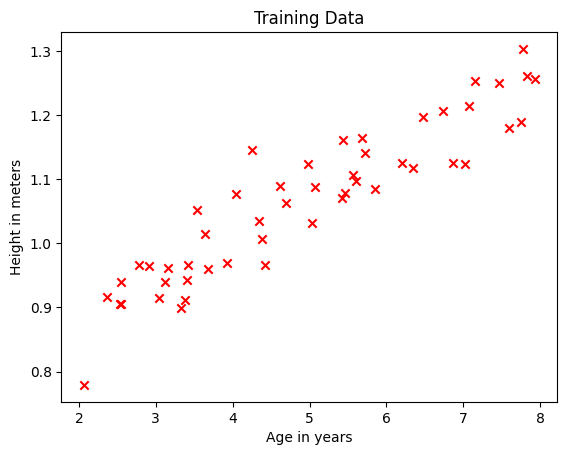
\includegraphics[width=0.6\textwidth]{img/plot_training_data}
        \caption{Gráfica de los datos de entrenamiento}
        \label{fig:plot_training_data}
    \end{figure}

%        Initialize the parameters to θ = 0�⃗. Run one iteration of gradient descent from this
%        initial starting point. Record the value of your parameters after this first
%        iteration. (20 pts)

    \subsection{Initialize the parameters to $\theta = 0$}\label{ssec:Initialize-Parameters}
    En este bloque de código se inicializan los parámetros $\theta$ a 0 y se ejecuta una iteración del algoritmo de descenso de gradiente.
    \begin {lstlisting}[language=Python, caption={Inicialización de los parámetros a $\theta = 0$},label={lst:InitializeParameters}]
# Initialize variables
m = len(X_train)      # Number of training examples
alpha = 0.07          # Learning rate
theta = np.zeros(2)   # Initial parameters

# Gradient descent iterations
for i in range(1):
# Predict heights based on current parameters
y_pred = theta[0] + theta[1] * X_train # hθ(x)= θ0 + θ1 * x

# Calculate the error
error = y_pred - y_train

# Update parameters using gradient descent algorithm
theta[0] -= alpha * (1/m) * np.sum(error)            # θ0:= θ0 - α *(1/m) ∑ [hθ(xi) - yi]
theta[1] -= alpha * (1/m) * np.sum(error * X_train)  # θ1:= θ1 - α *(1/m) ∑ [hθ(xi) - yi]*xi

# Print the parameters after one iteration
print('Theta0 after one iteration:', theta[0])
print('Theta1 after one iteration:', theta[1])

\end{lstlisting}
\noindent
Al ejecutar el código se obtuvieron los siguientes resultados:
\begin{itemize}
\item Theta0 after one iteration: 0.07452802382200001
\item Theta1 after one iteration: 0.38002167250780633
\end{itemize}

%Continue running gradient descent for more iterations until your parameters converge. Show your parameters final values
\subsection{Continue running gradient descent for more iterations}\label{ssec:Continue-Running-Gradient-Descent}
En este bloque de código se ejecutan 1000 iteraciones del algoritmo de descenso de gradiente.
\begin{lstlisting}[language=Python, caption={Ejecución de 1000 iteraciones del algoritmo de descenso de gradiente},label={lst:ContinueRunningGradientDescent}]
# Continue gradient descent for more iterations
for i in range(1000):
# Predict heights based on current parameters
y_pred = theta[0] + theta[1] * X_train # hθ(x)= θ0 + θ1 * x

# Calculate the error
error = y_pred - y_train

# Update parameters using gradient descent algorithm
theta[0] -= alpha * (1/m) * np.sum(error)            # θ0:= θ0 - α *(1/m) ∑ [hθ(xi) - yi]
theta[1] -= alpha * (1/m) * np.sum(error * X_train)  # θ1:= θ1 - α *(1/m) ∑ [hθ(xi) - yi]*xi

# Print the final parameter values
print('Final Theta0:', theta[0])
print('Final Theta1:', theta[1])
\end{lstlisting}
\noindent
Al ejecutar el código se obtuvieron los siguientes resultados:
\begin{itemize}
\item Final Theta0: 0.749921461773668
\item Final Theta1: 0.06392502646496022
\end{itemize}

%After convergence, plot the straight line fit from your algorithm on the same graph as your training data.
\subsection{Plot the straight line fit from your algorithm}\label{ssec:Plot-Straight-Line-Fit}
En este bloque de código se grafica la línea recta ajustada por los parámetros aprendidos por el algoritmo de descenso de gradiente.
Se grafican los datos de entrenamiento y la línea recta ajustada por los parámetros aprendidos por el algoritmo de descenso de gradiente.
Se muestra la relación entre la edad y la altura de los niños.

\begin{lstlisting}[language=Python, caption={Gráfica de la línea recta ajustada por el algoritmo de descenso de gradiente},label={lst:PlotStraightLineFit}]
# Plot the training data and the fitted line
plt.scatter(X_train, y_train, marker='x', c='r', label='Training Data')
plt.plot(X_train, theta[0] + theta[1] * X_train, color='b', label='Fitted Line')
plt.title('Training Data with Fitted Line')
plt.xlabel('Age in years')
plt.ylabel('Height in meters')
plt.legend()
plt.show()
\end{lstlisting}
\noindent
Al ejecutar el código se obtuvo la siguiente gráfica:
\begin{figure}[h]
\centering
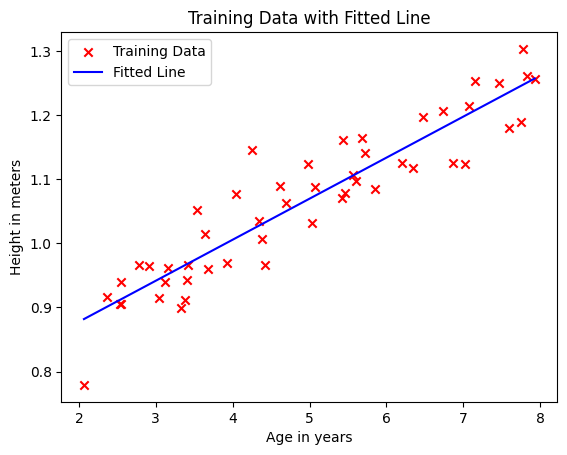
\includegraphics[width=0.6\textwidth]{img/plot_straight_line_fit}
\caption{Gráfica de la línea recta ajustada por el algoritmo de descenso de gradiente}
\label{fig:plot_straight_line_fit}
\end{figure}
%Finally, use your trained model to predict the height for two boys of age 3.5 and age 7. Show your results.
\subsection{Use your trained model to predict height   }\label{ssec:Predict-Height}
En este bloque de código se utilizan los parámetros aprendidos por el algoritmo de descenso de gradiente para predecir la altura de dos niños de 3.5 y 7 años.
\begin{lstlisting}[language=Python, caption={Predicción de la altura de dos niños de 3.5 y 7 años},label={lst:PredictHeight}]
# Predict heights for boys of age 3.5 and 7
age_3_5_height = theta[0] + theta[1] * 3.5
age_7_height = theta[0] + theta[1] * 7

# Print the predicted heights
print('Predicted height for a boy of age 3.5:', round(age_3_5_height,2))
print('Predicted height for a boy of age 7:', round(age_7_height,2))
\end{lstlisting}
\noindent
Al ejecutar el código se obtuvieron los siguientes resultados:
\begin{itemize}
\item Predicted height for a boy of age 3.5: 0.97
\item Predicted height for a boy of age 7: 1.2
\end{itemize}

\clearpage
\section{Conclusiones}
\noindent
En este informe se presentó el trabajo realizado en el laboratorio 3 de Redes Neuronales Convolucionales.
Se implementaron varios bloques de código relacionados con el uso de la regresión lineal y el algoritmo de descenso de gradiente.
se ejemplificó el uso de la regresión lineal para predecir la altura de varios niños basándose en sus edades.
Se utilizó una tasa de aprendizaje de $\alpha = 0.07$ y se realizaron 1000 iteraciones del algoritmo de descenso de gradiente.
Se graficaron los datos de entrenamiento y la línea recta ajustada por los parámetros aprendidos por el algoritmo de descenso de gradiente.
Se utilizó el modelo entrenado para predecir la altura de dos niños de 3.5 y 7 años.

\end{document}
